\documentclass[10pt]{article}
\usepackage[total={170mm,230mm}]{geometry}

\usepackage{cmap}
\usepackage{hyperref}
\usepackage[utf8]{inputenc}
\usepackage[T2A]{fontenc}
\usepackage[russian]{babel}

\usepackage{graphicx}
\usepackage{xcolor}
\usepackage{amssymb}
\usepackage{amsfonts}
\usepackage{amsmath}
\usepackage{amsthm}
\usepackage{physics}
\usepackage{wrapfig}
\usepackage{cancel}
\usepackage{pdfpages}
\usepackage{hyperref}
% \usepackage{bibtex}

\title{Домашнее задание №1}
\author{Александр Козлов}
\date{\today}

\begin{document}

\maketitle

\section*{Формулировка задания}

Дан гамильтониан одномерной квантово-механической системы с потенциалом в виде гауссовой ямы
\begin{equation}
    H = - \dv[2]{}{x} + V_0\, e^{-x^2},
\end{equation}
где $V_0 < 0$. Требуется сделать следующее.

\begin{enumerate}
    \item Найти константы связи $V_0$, при которых в системе возникает одно, два и три связанных состояния.

    \item Исследовать зависимость вычислительных затрат от размера сетки.

    \item Исследовать зависимость погрешности энергий состояний от размера сетки и границ бокса.
\end{enumerate}

\section{Численное решение}

Рассматриваемое уравнение Шрёдингера (УШ) имеет вид
\begin{equation}
    -\dv[2]{\psi}{x} + V_0\, e^{-x^2}\, \psi  = E\, \psi
    \label{eq:SE}
\end{equation}
или
\begin{equation}
    \dv[2]{\psi}{x}  + (E - V_0\, e^{-x^2})\, \psi  = 0.
\end{equation}
Стоит заметить, что такое уравнение соответствует обычному одномерному УШ при $\hbar=1$ и $m=1/2$. 

Прежде всего зададим равномерную сетку
\begin{equation}
    x_0 = -R,\; x_1 = x_0 + \delta,\; x_2 = x_0 + 2\delta,\; \ldots,\; x_k = x_0 + k\delta,\; \ldots,\; x_M = x_0 + M \delta = R
\end{equation}
с шагом $\delta = 2R/M$, где $M$~---~целое положительное число, а $R$~---~положительное действительное число. Будем пользоваться численной аппроксимацией второй производной
\begin{equation}
    \dv[2]{\psi}{x}(x_k) = \dfrac{\psi(x_{k+1}) - 2\psi(x_{k}) + \psi(x_{k-1})}{\delta^2} + O(\delta^2),\quad k = \overline{1,M-1}
\end{equation}
и сводить уравнение \eqref{eq:SE} к задаче диагонализации трёхдиагональной матрицы. 

Перед тем, как писать явный вид такой матрицы, необходимо поговорить о том, как будут задаваться граничные условия. Ясно, что волновые функции состояний дискретного спектра будут экспоненциально затухать при больших по абсолютному значению $x$. Это обстоятельство может быть численно учтено различными вариантами, однако, остановимся на варианте, при котором полагается $\psi(x_0) = \psi(x_M) = 0$. Тогда численное приближение УШ для $k=1$ примет вид
\begin{equation}
    -\dfrac{\psi(x_{2}) - 2\psi(x_{1})}{\delta^2} + V(x_1)\,\psi(x_1) = E\psi(x_1).
\end{equation}
Для $k=M-1$ получаем аналогичное уравнение
\begin{equation}
    -\dfrac{-2\psi(x_{M-1})+\psi(x_{M-2}) }{\delta^2} + V(x_{M-1})\,\psi(x_{M-1}) = E\psi(x_{M-1}).
\end{equation}
А для всех остальных $k$ имеем уравнение
\begin{equation}
    -\dfrac{\psi(x_{k+1}) - 2\psi(x_{k}) + \psi(x_{k-1})}{\delta^2} + V(x_k)\,\psi(x_k) = E\psi(x_k).
\end{equation}
В матричном виде задача записывается так:
\begin{equation}
\begin{split}
    &\begin{pmatrix} 
        2\delta^{-2}+V(x_1)& -\delta^{-2}\\
        -\delta^{-2}& 2\delta^{-2}+V(x_2)& -\delta^{-2}\\
        % & -\delta^{-2}& 2\delta^{-2}+V_0\,e^{-x_3^2}& -\delta^{-2}\\
        & & & \ddots&\\
        & & & & -\delta^{-2}& 2\delta^{-2}+V(x_{M-2})& -\delta^{-2}\\
        & & & & & -\delta^{-2}& 2\delta^{-2}+V(x_{M-1})
    \end{pmatrix}
    \begin{pmatrix}
        \psi(x_1)\\
        \psi(x_2)\\
        \vdots\\
        \psi(x_{M-2})\\
        \psi(x_{M-1})
    \end{pmatrix}\\
    &=E
    \begin{pmatrix}
        \psi(x_1)\\
        \psi(x_2)\\
        \vdots\\
        \psi(x_{M-2})\\
        \psi(x_{M-1})
    \end{pmatrix}.
\end{split}
\end{equation}
Таким образом надо диагонализовать симметричную трёхдиагональную матрицу размера $(M-1)\times(M-1)$.

\section{Количество связанных состояний в зависимости от константы связи}

При размере сетки $M=10\, 000$ и ширине бокса $R=15$ была получена зависимость числа связанных состояний от параметра связи, показанная на Рис. \ref{fig:n_vs_v0}.
\begin{figure}[htbp]
    \centering
    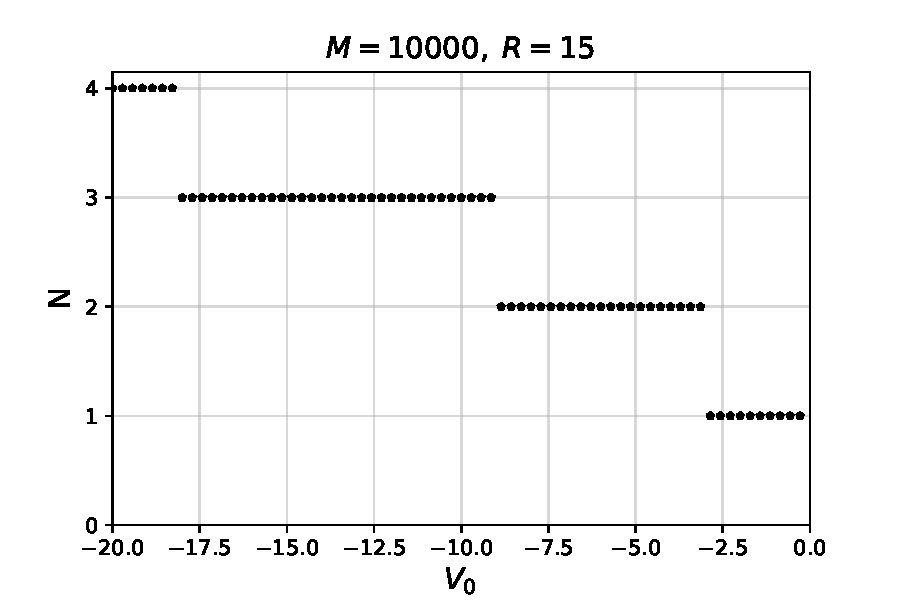
\includegraphics[width=0.5\textwidth]{../figures/num_eigen_vs_v0}
    \caption{Количество связанных состояний $N$ в зависимости от константы связи $V_0$ при размере сетки $M=10\, 000$ и ширине бокса $R=15$. Вертикальными линиями отмечены границы, адаптированные из работы \cite{article}.}
    \label{fig:n_vs_v0}
\end{figure}
Для оценки правильности полученных результатов обратимся к работе \cite{article}, где рассматривается уравнение, похожее на нашее за исключением того, что $v_0$ в статье соответсует $-V_0/2$ у нас. Если учесть разницу в обозначениях, то можно вынести из данной работы, что одно связанное состояние существует при $0 < \abs{V_0} < 2.684$, два связанных состояния --- при $2.684 < \abs{V_0} < 8.650$, три состояния --- при $8.650 < \abs{V_0} < 17.796$. 


\section{Зависимость времени работы программы от размера сетки}

Определим, как долго работает программа при различных значениях параметра $M$ --- размера сетки. Для определённости фиксируем прочие параметры задачи, например, положим их следующими: $V_0 = -1.0$ и $R=6$. Результаты продемонстрированы на Рис. \ref{fig:T_vs_M}.
\begin{figure}[htbp]
    \centering
    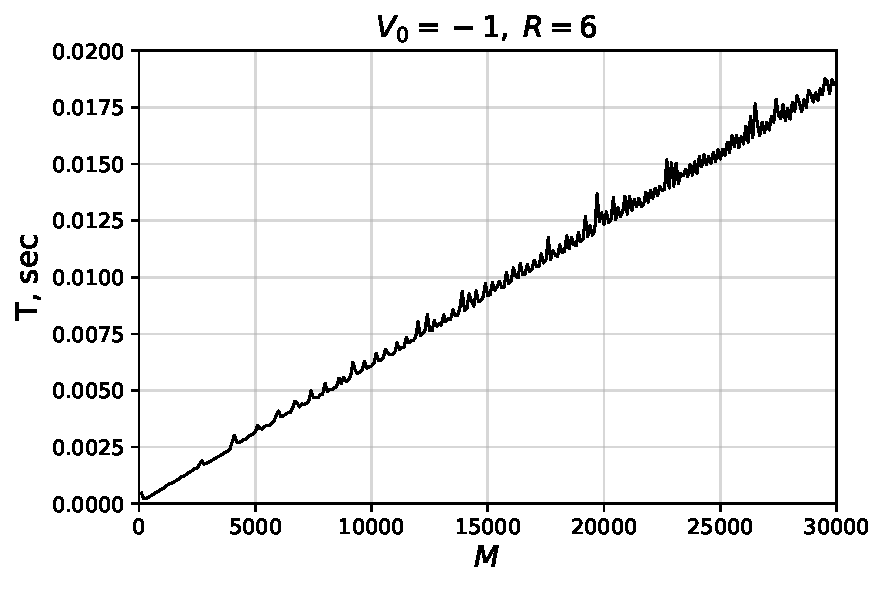
\includegraphics[width=0.5\textwidth]{../figures/T_vs_M}
    \caption{Время работы программы $N$ в секундах в зависимости от размера сетки $M$ при $V_0 = -1.0$ и $R=6$.}
    \label{fig:T_vs_M}
\end{figure} 

\section{Зависимость ошибки определения уровней энергии от размера сетки и размера бокса}

Рассмотрим случай $\abs{V_0}=1$. Для такого случая вариационный метод даёт оценку $E_1 = -0.335$. В качестве наиболее точного значения энергии основного состояния возьмем значение, получаемое в пределе $M\rightarrow \infty$, для чего аппроксимируем параболлой зависимость уровня энергии от $1/M$. Для $R=12$ было получено, что наиболее точное значение энергии основного состояния есть $E_1 = -0.3539907385825565$. Такое экстраполированное значение было взято за эталон. На Рис. \ref{fig:abserr} представлены результаты расчётов.
\begin{figure}[htbp]
    \centering
    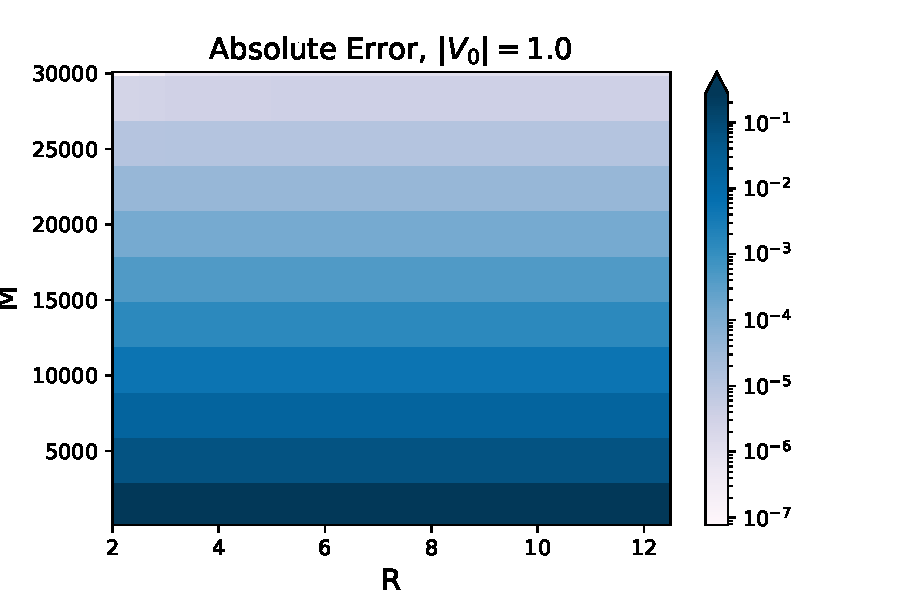
\includegraphics[width=0.5\textwidth]{../figures/abserr}
    \caption{Абсолютная ошибка вычисления энергии основного состояния при различных размерах сетки $M$ и бокса $R$ для случая $\abs{V_0}=1$.}
    \label{fig:abserr}
\end{figure}

Рассмотрим случай $\abs{V_0}=5$, когда имеется два связанных состояния. В качестве наиболее точных значений энергии состояний рассмотрим значения, получаемые экстраполяцией для предела $M\rightarrow \infty$: $E_1=-3.140334020243438,\; E_2= -0.40611998906602725$. На Рис. \ref{fig:abserr_v0_5} представлены результаты расчётов.
\begin{figure}[htbp]
    \centering
    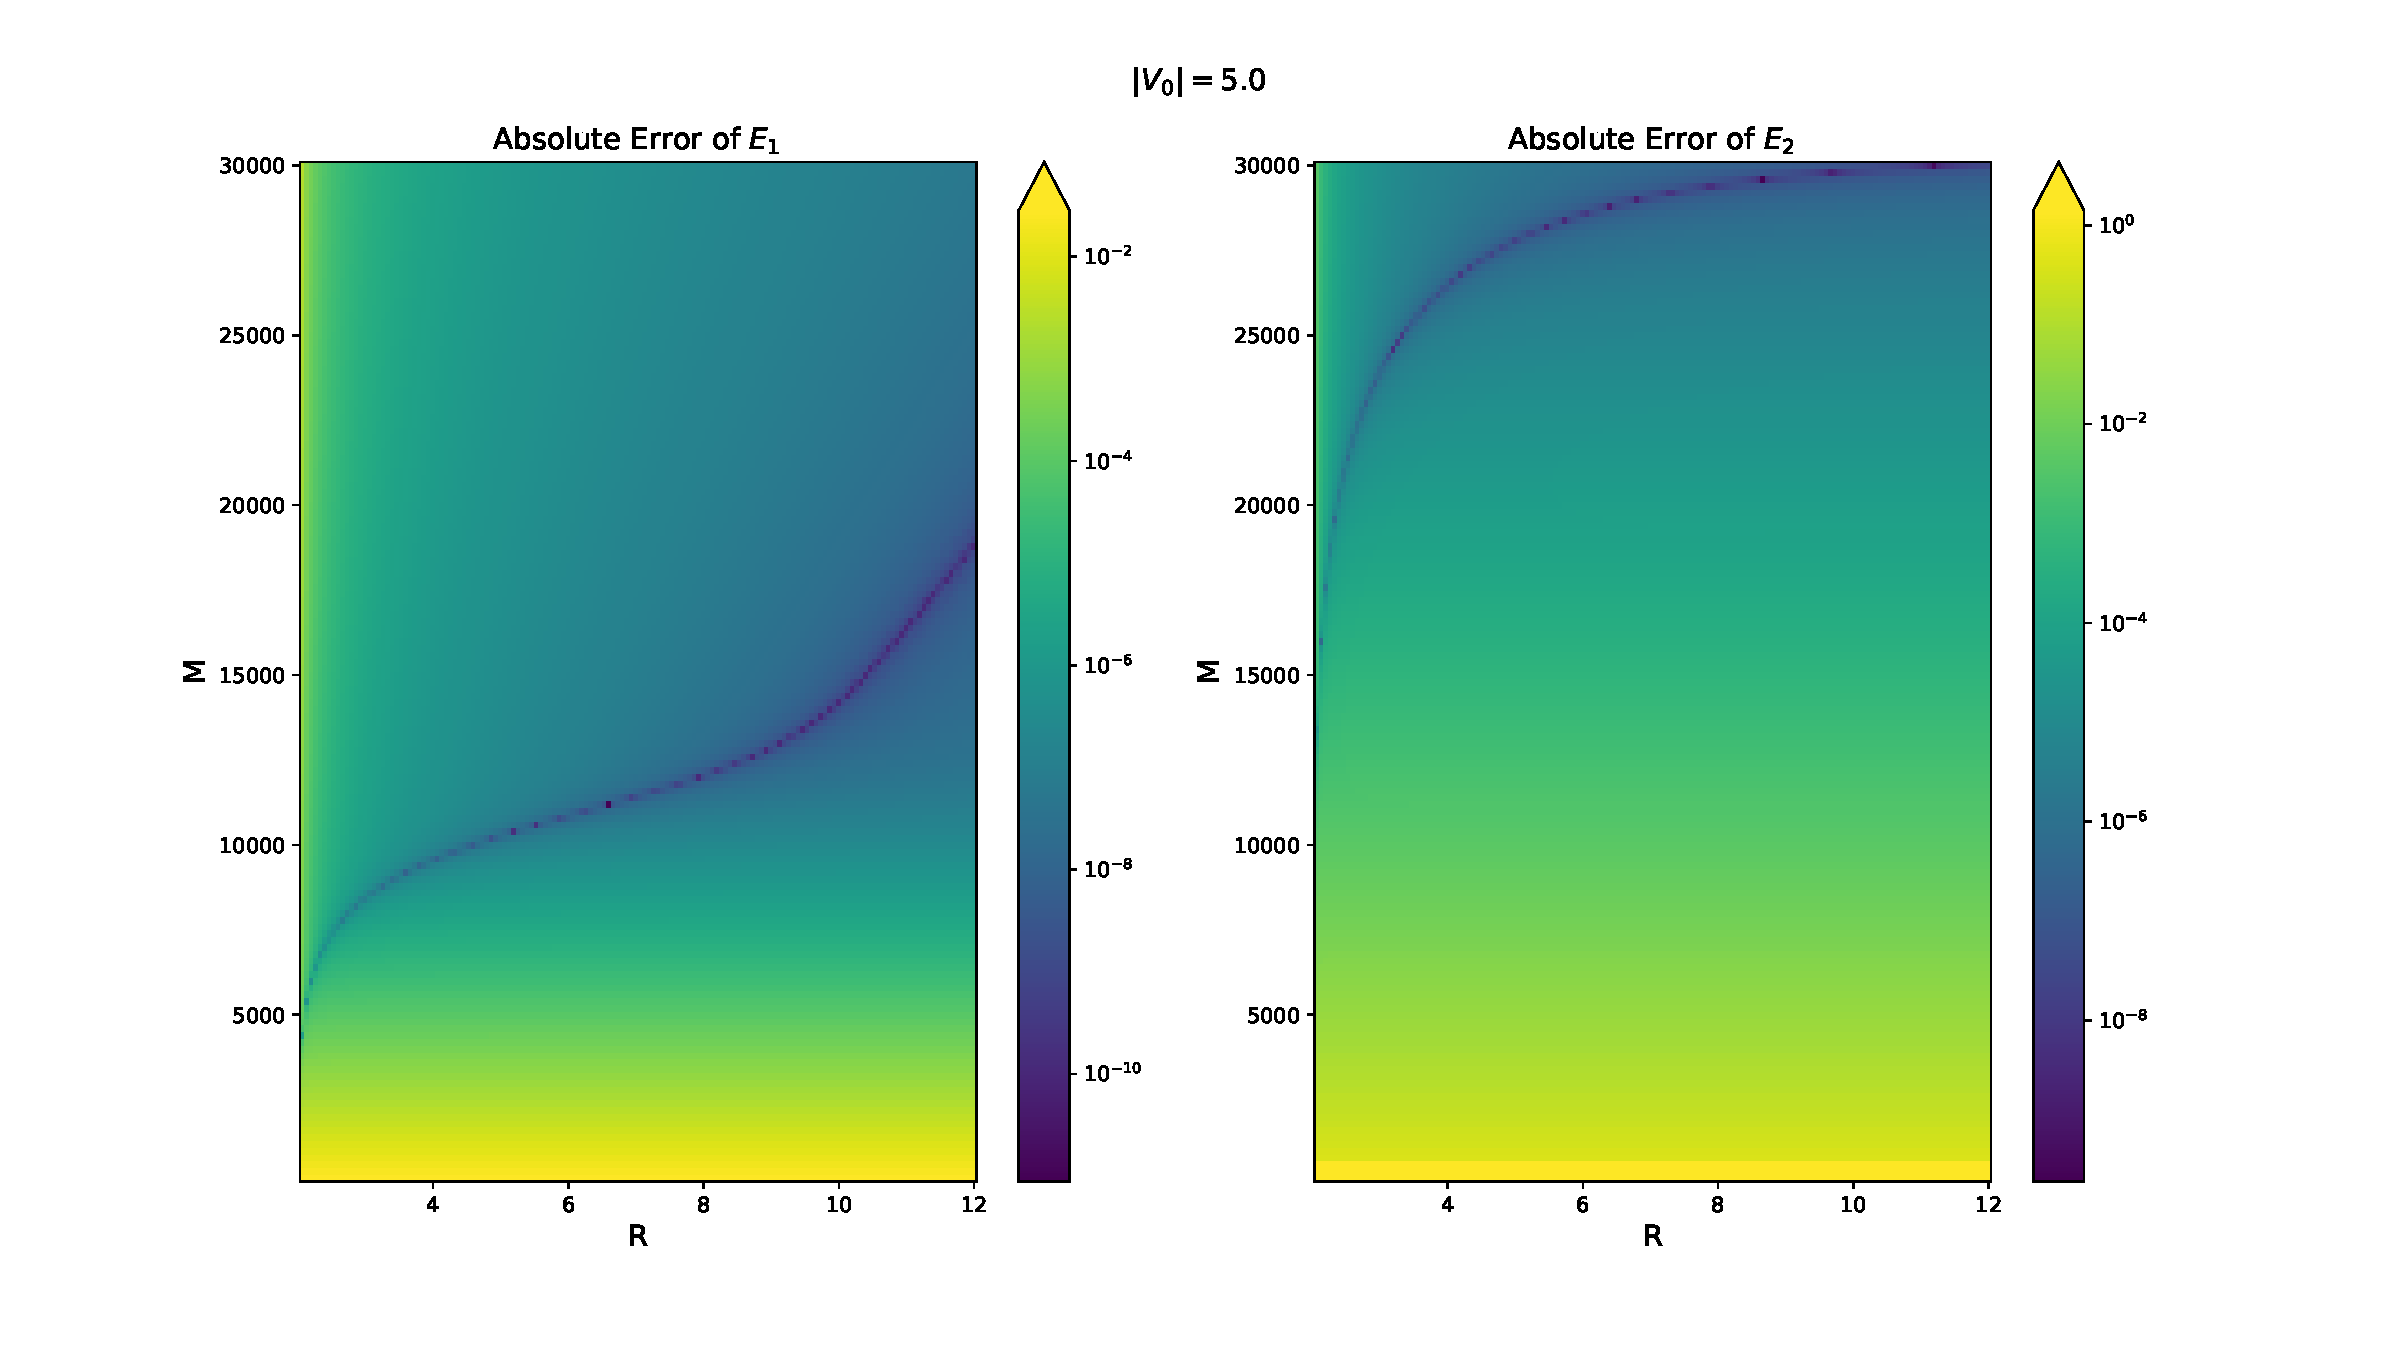
\includegraphics[width=\textwidth]{../figures/abserr_v0_5}
    \caption{Абсолютные ошибки вычисления энергий дискретного спектра при различных размерах сетки $M$ и бокса $R$ для случая $\abs{V_0}=5$.}
    \label{fig:abserr_v0_5}
\end{figure}

\begin{thebibliography}{10}
    \bibitem{article}
    Fernández, Francisco.
    \newblock Quantum Gaussian wells and barriers.
    \newblock {\em Amer. \ J. \ Phys.}, 79:752--754, 2011.
\end{thebibliography}

\end{document}
